\section{Theorie}

\textbf{\underline{Ziel:}}
Die folgenden Größen sollen bestimmt werden:
\begin{itemize}
  \item der effektive Dämpfungswiderstand $R_\text{eff}$ des Systems.
  \item Abklingdauer $T_\text{ex}$, nach der die Spannung im RLC-Kreis auf den $e$-ten Teil ihrer Amplitude abgefallen ist.
  \item der Widertand $R_\text{ap}$, bei dem der aperiodische Grenzfall eintritt.
  \item Frequenzabhängigkeit der Spannung.
  \item Phasenverschiebung zwischen der Kondensatorspannung $U_\text{C}$ und der externen Erregerspannung $U_\text{Err}$
  in Abhängigkeit der Frequenz.
\end{itemize}
\subsection{Gedämpfter RLC-Kreis}
\begin{figure}
  \centering
  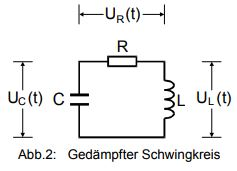
\includegraphics{Text/Gedaempfter_RLC-Kreis.JPG}
  \caption{Gedämpfter RLC-Kreis \cite[284]{sample}}
  \label{fig:Aufbau1}
\end{figure}
Betrachtet wird zunächst ein einfacher RLC-Kreis. Ist in diesem eine Energiemenge eingespeichert, so wird die Energie zwischen
den beiden Energiespeichern - der Kapazität $C$ und der Induktivität $L$ - hin und her transportiert.
Allerdings wirkt der Widerstand $R$ hier als Dämpfung, sodass ein Teil der Energie immer in Wärme umgewandelt wird und somit
nach einer gewissen Zeit kein Strom mehr fließt.
Mit der zweiten Kirchhoff'schen Regel lässt sich somit folgene Gleichung aufstellen:
\begin{equation}
  0=U_R+U_C+U_L
\end{equation}
Dabei gilt:
\begin{align*}
  U_R&=RI & U_C&=\frac{Q}{C} & U_L&=L\dot{I}
\end{align*}
Daraus ergibt sich folgende Differentialgleichung:
\begin{equation}
  \ddot{I}+\frac{R}{L}\dot{I}+\frac{1}{LC}I=0
\end{equation}
Der Exponentialansatz liefert die Lösung der Differentialgleichung:
\begin{equation}
  I=e^{-2\pi \mu t}\cdot \left(A_1 e^{i2\pi \nu t}+A_2 e^{-i2\pi \nu t}\right)
  \label{eqn:lsg}
\end{equation}
Dabei sind $\mu=\frac{R}{4\pi L}$  und  $\nu = \frac{1}{2\pi}\cdot \sqrt{\frac{1}{LC} - \frac{R^2}{4L^2}}$.
Für ein reelles $\nu$ gilt $\frac {1}{LC} > \frac{R^2}{4L^2}$ und die Differentialgleichung lässt sich schreiben als:
\begin{equation}
  I(t) = A_0 \cdot e^{-2 \pi\mu t}\cdot cos{(2\pi\nu t+ \phi_o)}
\end{equation}
Daraus lässt sich die Abklingzeit
\begin{equation}
  T_\text{ex}=\frac{1}{2\mu \pi} =\frac{2L}{R}
  \label{eqn:tex}
\end{equation}
ablesen. Ist $\nu$ jedoch imaginär, so ist
\begin{equation}
  I \sim e^{-(2\pi \mu - i2\pi \nu)t},
\end{equation}
wobei der Exponent nun auf Grund $\nu$ reell ist.
Da es sich hierbei um eine Exponentialfunktion mit negativem
Vorzeichen im Exponent handelt, fällt sie stark.
Am schnellsten fällt die Funktion jedoch, wenn $\nu=0$, also wenn
\begin{equation}
\frac{1}{LC}=\frac{R^2_\text{ap}}{4L^2}
\label{eqn:ap}
\end{equation}
ist.
Dieser Fall wird als aperiodischer Grenzfall bezeichnet.
\subsection{Angeregter RLC-Kreis}
\begin{figure}
  \centering
  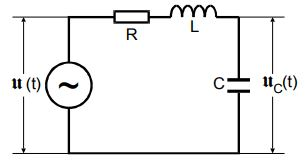
\includegraphics{Text/Angeregter_RLC-Kreis.JPG}
  \caption{Angeregter RLC-Kreis \cite[289]{sample}}
  \label{fig:Aufbau2}
\end{figure}
Zunächst wird ein Wechselstromgenerator an den RLC-Kreis angeschlossen. Die Differentialgleichung
\begin{equation}
  LC\ddot{U}_C+RC\dot{U}_C+U_C=U_0e^{i\omega t}
\end{equation}
beschreibt den Spannungsverlauf des Kondensators und wird gelöst durch
\begin{equation}
  U_C=\frac{U_0(1-LC\omega^2-i\omega RC)}{(1-LC\omega^2)^2+\omega^2R^2w^2}
\end{equation}
Die Phasenverschiebung zur Erregerspannung $U_\text{Err}$ ist gegeben durch:
\begin{equation}
  \phi(\omega)=\arctan{\left(\frac{Im(U)}{Re(U)}\right)}=\arctan{\left(\frac{-\omega RC}{1-LC\omega^2}\right)}
\end{equation}
Für die Phasen $\phi_1=\frac{\pi}{4}$ und $\phi_2=\frac{3\pi}{4}$ ergeben sich folgende $\omega$:
\begin{align}
  \omega_1 &= \frac{R}{2L}+\sqrt{\frac{R^2}{4L^2}+\frac{1}{LC}}\\
  \omega_2 &= -\frac{R}{2L}+\sqrt{\frac{R^2}{4L^2}+\frac{1}{LC}}
  \label{eqn:omegas}
\end{align}
Eine weitere wichtige Größe ist die Resonanzfrequenz, also die Frequenz, für die $U_C$ maximal wird.
Um diese zu erhalten, muss zunächst der Betrag der Spannung $U_C$ in Abhängigkeit von $\omega$ gebildet werden:
\begin{equation}
  \lvert U_C(\omega)\rvert=\frac{U_0}{\sqrt{\left(1-LC\omega^2 \right)^2+\omega^2R^2C^2}}
\label{eqn:U_Omega}
\end{equation}
An dieser Gleichung lässt sich erkennen, dass $\underset{\omega \to \infty}{\lim} \lvert U_C(\omega)\rvert =0$
und $\underset{\omega \to 0}{\lim} \lvert U_C(\omega)\rvert=U_0$ sind. Ebenfalls lässt sich mit ihr die Resonanzfrequenz bestimmen:
\begin{equation}
  \omega_\text{res}=\sqrt{\frac{1}{LC}-\frac{R^2}{2L^2}}
  \label{eqn:ores}
\end{equation}
Wird nun der Fall $\frac{1}{LC} \gg \frac{R^2}{2L^2}$ betrachtet, erhält man die Kreisfrequenz $\omega_0$ des LC-Schwingkreises
\begin{equation}
  \omega_0=\sqrt{\frac{1}{LC}}
  \label{eqn:omega0}
\end{equation}
Ist dies tatsächlich der Fall, so gilt
\begin{equation}
  U_\text{C,max}=q \cdot U_\text{Err},
\end{equation}
wobei der Faktor q als Güte bezeichnet wird und wie folgt definiert ist:
\begin{equation}
  q=\frac{1}{\omega_0 RC}
  \label{eqn:q}
\end{equation}
Eine weitere wichtige Eigenschaft der Gleichung \eqref{eqn:U_Omega} ist die Breite der Resonanzkurve.
Für diese werden $\omega_+$ und $\omega_-$, die, wenn sie in Gleichung \eqref{eqn:U_Omega} eingesetzt werden, den Betrag
der Amplitude um den Faktor $\sfrac{1}{\sqrt{2}}$ verringern, benötigt.
Wenn $\frac{R^2}{L^2} \ll \omega^2_0$ ist, gilt für die Breite der Resonanzkurve:
\begin{equation}
  \omega_+ - \omega_- \approx \frac{R}{L}
  \label{eqn:bres}
\end{equation}
Im Falle einer schwachen Dämpfung gilt dabei zusätzlich:
\begin{align}
  \omega_+ - \omega_- = \omega_1 - \omega_2
\end{align}
